\documentclass{article}

\usepackage{times}
\usepackage{amssymb, amsmath, amsthm}
\usepackage[margin=1in]{geometry}
\usepackage{graphicx}

\begin{document}

\title{MTH 311 Homework 8}
\author{Philip Warton}
\date{\today}
\maketitle

\section*{4.4.9}
\subsection*{(a)}
Show that a Lipschitz function is uniformly continuous.
\begin{proof}
Suppose $f: A \rightarrow \mathbb{R}$ is a Lipschitz function, i.e. there exists $M>0$ such that
\[ \left|\frac{f(x)-f(y)}{x-y}\right| \leqslant M\]
for all $x \neq y \in A$. We can multiply the above inequality and get $|f(x)-f(y)| \leqslant M |x-y|$. Let $\epsilon > 0$ be arbitrary, and let $\delta = \dfrac{\epsilon}{M}$. Then if we have $|x-y| < \dfrac{\epsilon}{M}$, we can mutliply by $M$ and get 
\[ |f(x)-f(y)| \leqslant M|x-y| < M \delta = M \dfrac{\epsilon}{M} = \epsilon\]
\end{proof}

\subsection*{(b)}
Is the converse true? No.
\begin{proof}
Take the funciton $f(x) = \sqrt{x}$ on $[0,1]$. We say that it is uniformly continuous because it is continuous on a compact set. Now, since the definition must apply for all $x,y \in A$ choose $x = \dfrac{1}{n} \in [0,1]$ which works for any $n \in \mathbb{N}$ and $y = 0$. Then
\[ \left| \frac{f(\frac{1}{n}) - f(0)}{\frac{1}{n}}\right| = \sqrt{n}\] 
Since $\sqrt{n}$ is not bounded we say that the function is not Lipschitz.
\end{proof}

\section*{4.5.5 b}
\begin{proof}
We continue this proof from where the book left off. We have an interval $I_1 = [a_1, b_1]$ such that $f(a_1) < 0$ and $f(b_1) \geqslant 0$. We generalize the process by taking $z_n = \frac{a_n + b_n}{2}$, and then if $f(z_n) > 0$ then $b_{n+1} = z_n$. If $f(z_n) < 0$ then $a_{n+1} = z_n$. Otherwise, $z_n \in [a,b]$ and $f(z_n) = 0$, and we are done. By the inductive step, we assume that we have $I_n = [a_n, b_n]$, where $f(a_n) < 0$ and $f(b_n) > 0$. Then, we can find a midpoint $z_n$ and create the interval $I_{n+1}$ such that $f(a_{n+1}) < 0$ and $f(b_{n+1}) > 0$. \\\\
We say that the length of this interval is equal to $\frac{a-b}{2^n}$, since each time $n$ increases by one we cut the interval in half. Then we take the sequence of intervals $I_n$ for all $n \in \mathbb{N}$, and it follows that the length of $I_n$ approaches 0. Since the length of $I_n$ approaches zero, and by the Nested Interval Property the infinite intersection of $I_n$ is non-empty, we say that there is exactly one number $c$ such that $\bigcap_{n \in \mathbb{N}}I_n = \{c\}$. \\\\
Suppose that $f(c) > 0$. Then there would be some $n \in \mathbb{N}$ such that $f(I_n) > 0$ i.e. $f(a_n) > 0$ and $f(b_n) > 0$. This is not possible by the process in which we chose $f(a_n)$, therefore $c \leqslant 0$. Now suppose $f(c) < 0$. Then, similarly there must be some interval where $f(b_n) < 0$, which again is not possible. Thus $f(c )\geqslant 0$. Since we have shown $f(c)$ not to be strictly positive or strictly negative, it follows that $f(c) = 0$.
\end{proof}

\section*{5.2.5}
\subsection*{(a)}
The function $f$ is continuous at 0 for $|a| \geqslant 1$.
\begin{proof}
0 is a limit point of $[0, \infty)$. Thus, we can use the functional limit characterization of continuity and say that if $lim_{x \rightarrow 0}f(x) = f(0)$ then $f$ is continuous at 0. Suppose $|a| <1$. Then for all $a \neq 0$, this limit is undefined. For $a=0$, the limit is equal to $1 \neq 0$. Therefore $a$ must be greater than or equal to 1. Assume that $a \geqslant 1$, then $lim_{x \rightarrow 0}x^a = 0 = f(0)$. Therefore the function is continuos at $0$ assuming $a \geqslant 1$.
\end{proof}

\subsection*{(b)}
$a >1$.

\section*{5.2.7}
\begin{proof}
\end{proof}

\section*{5.3.1 a}
\begin{proof}
Suppose $f$ is differentiable on $[a,b]$ and $f'$ is continuous on $[a,b]$. Without loss of generality, let $x < y \in [a,b]$. Then choose the interval $[x,y] \subset [a,b]$. Then by the mean value theorem there exists $c \in [x,y]$ such that $f'(c) = \dfrac{f(x)-f(y)}{x-y}$. Since $f'$ is continuous on the compact set $[a,b]$ we say that there exists $M>0$ such that $f'(x) \leqslant M$. Therefore we have
\[ \frac{f(x) - f(y)}{x-y} = f'(c) \leqslant M \]
And we say that $f$ is Lipschitz.
\end{proof}

\section*{5.3.5 b}
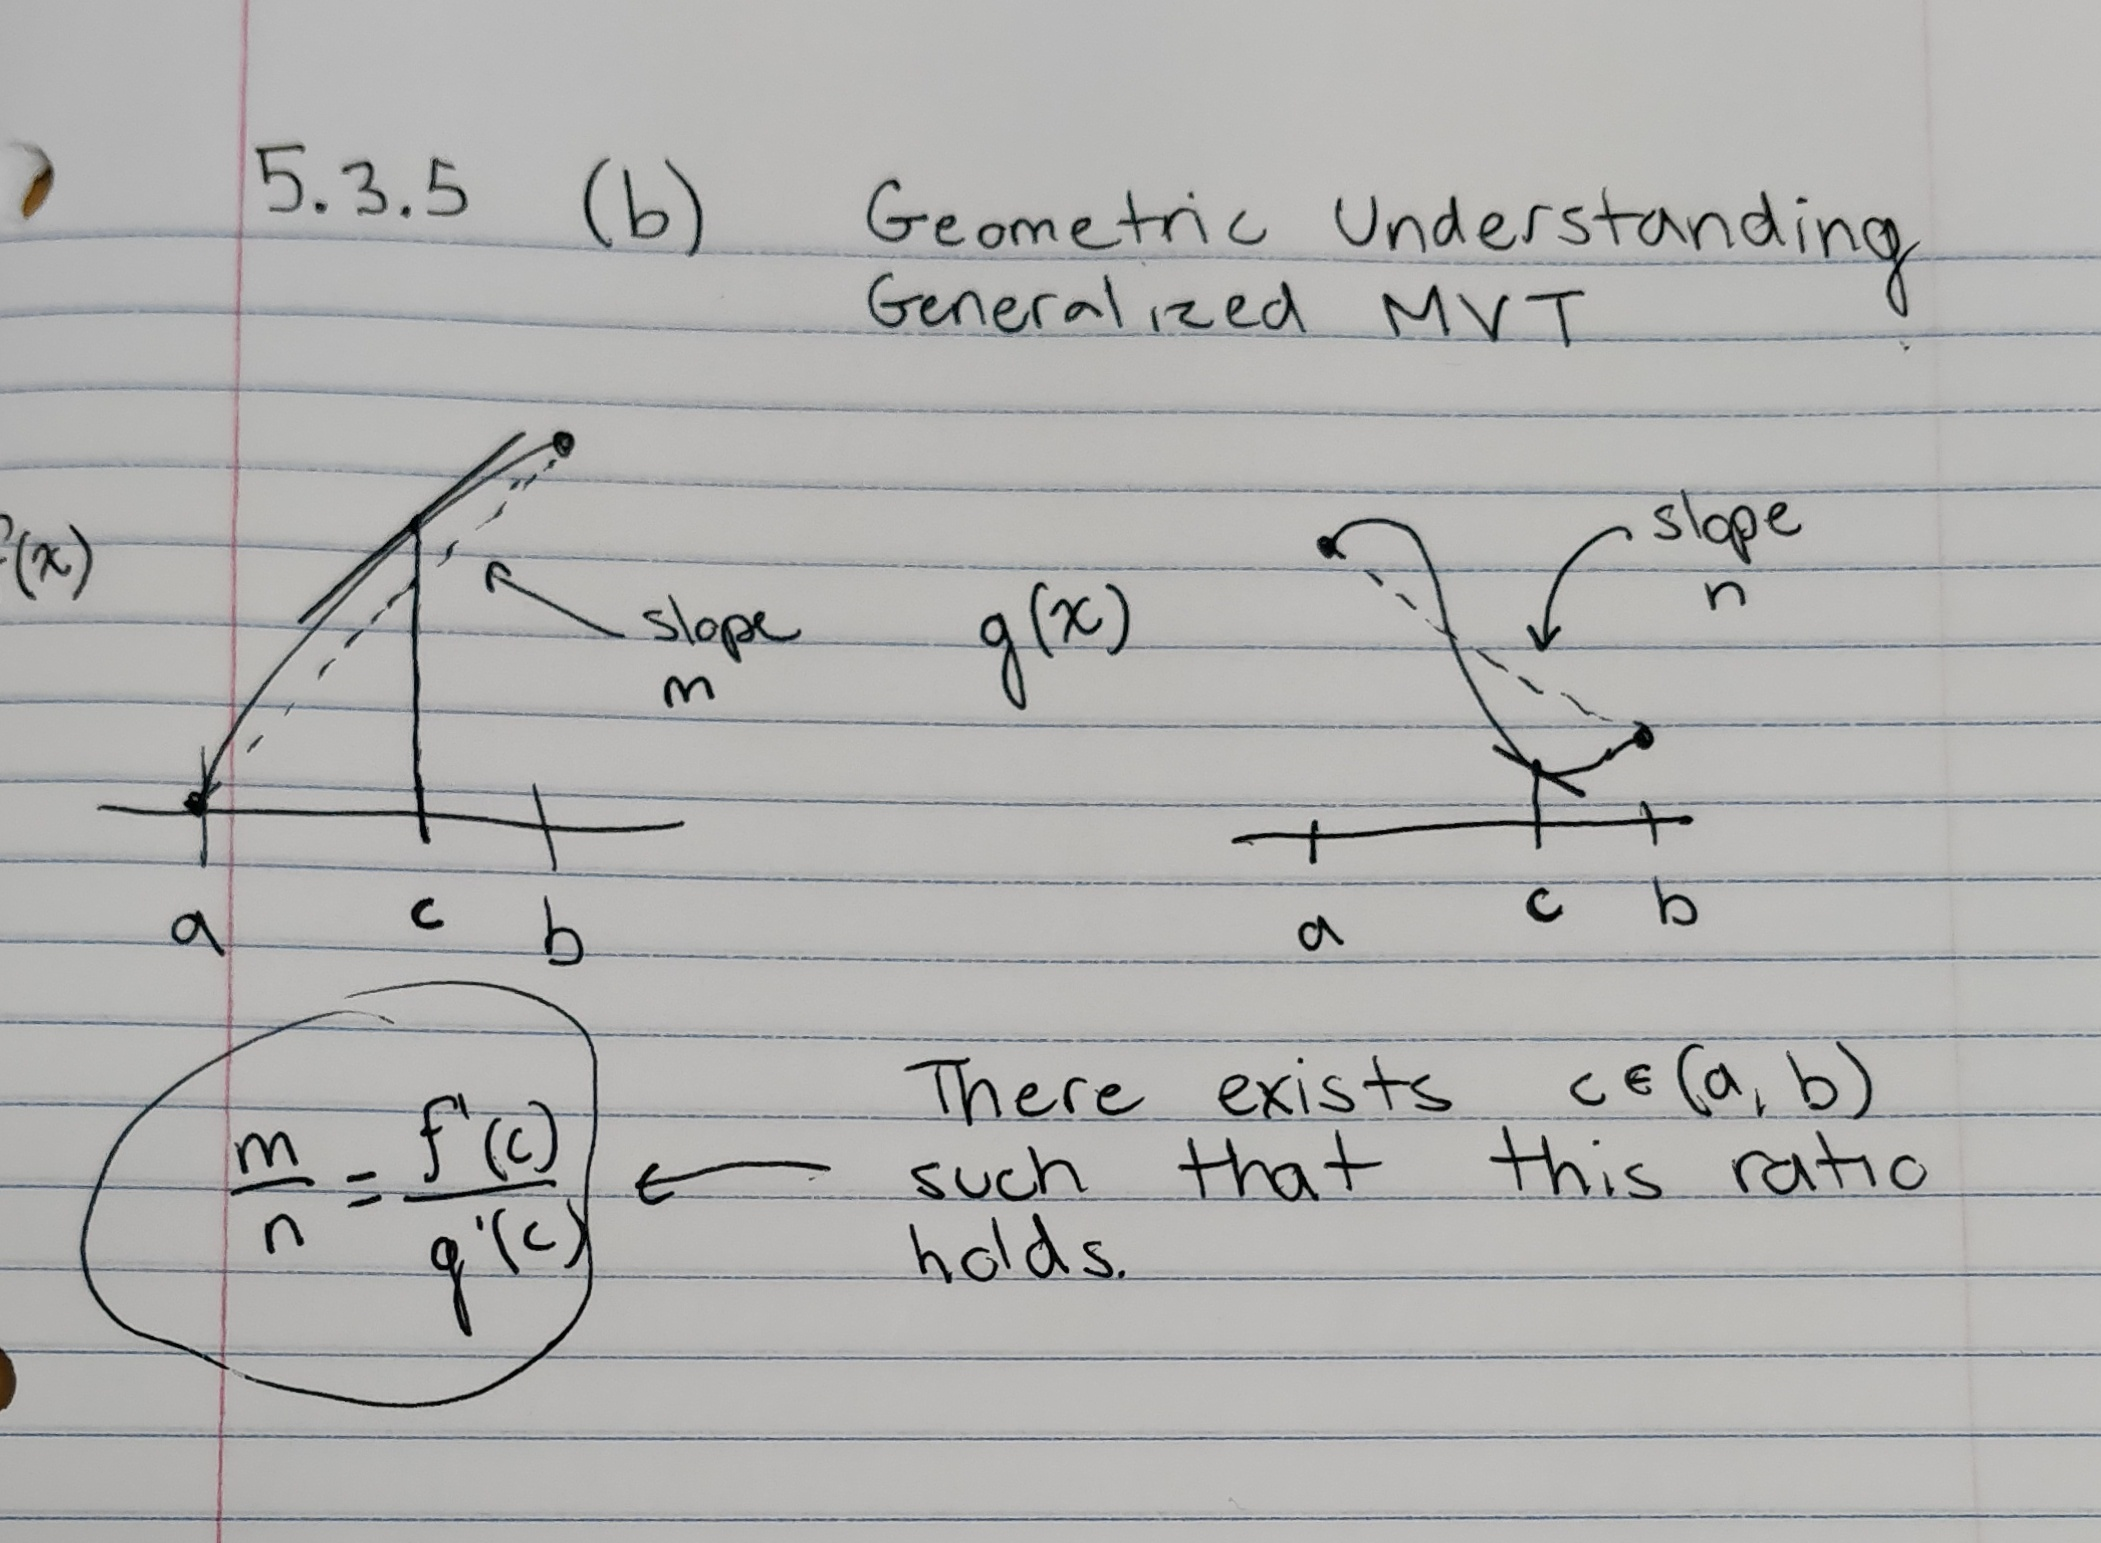
\includegraphics[scale=0.1]{pic.jpg}

\end{document}